\section{Abjad's object model}

\begin{frame}{Object model}
    \begin{block}
        {Abjad models musical score as a tree of components}
        Containers, leaves, spanners \& indicators
    \end{block}
    \begin{block}
        {Relationships between objects are modeled explicitly}
        Parentage, lineage, logical tie, logical voice
    \end{block}
    \begin{block}
        {Primitive objects are also modeled explicitly}
        Duration, Offset, Pitch, PitchClass, Interval, Octave, Accidental
    \end{block}
    \begin{block}
        {Top-level functions expose higher-level interfaces}
        Inspection, iteration, selection, mutation, persistence
    \end{block}
\end{frame}

\begin{frame}{Containers, leaves \& spanners}
    \begin{figure}
    \begin{centering}
        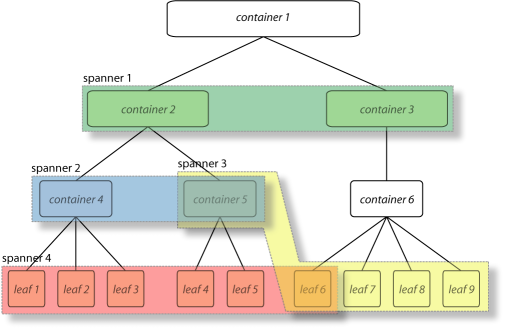
\includegraphics[height=2.5in]{assets/include-container-spanner.png}
    \caption{Spanners introducing cyclicity}
    \end{centering}
    \end{figure}
\end{frame}

\begin{frame}[fragile]{Parsers}
\begin{markdown}
- PLY-powered
- Pervasive throughout the system
- LilyPond syntax parsing
    - Includes a Scheme parser for LilyPond's embedded Scheme-Lisp
- IRCAM-inspired RTM-parsing
- *Reduced-LilyPond*-parsing for pedagogical examples
\end{markdown}
\end{frame}

\begin{frame}[fragile]{A two voice example}
\begin{comment}
<abjad>
upper_staff_string = "abj: | 5/8 c'8 r8 d'4 e'8 || 7/8 e'8 r8 fs'2 g'8 |"
lower_staff_string = "abj: | 5/8 c4. b8 r8 || 7/8 a8 af8 bf8 c'4 b4 |"
upper_staff= Staff(upper_staff_string, name='Upper Staff')
lower_staff = Staff(lower_staff_string, name='Lower Staff')
staff_group = StaffGroup([upper_staff, lower_staff], name='Staff Group')
score = Score([staff_group], name='Score')
</abjad>
\end{comment}

\begin{abjadbookoutput}
\begin{singlespacing}
\vspace{-0.5\baselineskip}
\begin{minted}{pycon}
>>> upper_staff_string = "abj: | 5/8 c'8 r8 d'4 e'8 || 7/8 e'8 r8 fs'2 g'8 |"
>>> lower_staff_string = "abj: | 5/8 c4. b8 r8 || 7/8 a8 af8 bf8 c'4 b4 |"
>>> upper_staff= Staff(upper_staff_string, name='Upper Staff')
>>> lower_staff = Staff(lower_staff_string, name='Lower Staff')
>>> staff_group = StaffGroup([upper_staff, lower_staff], name='Staff Group')
>>> score = Score([staff_group], name='Score')
\end{minted}
\end{singlespacing}
\end{abjadbookoutput}

\end{frame}

\begin{frame}[fragile]{Top-level functions}
    \begin{block}{show(), play() and graph()}
        \emph{Illustratable} visualization or sonification
    \end{block}
    \begin{block}{attach(), detach()}
        Indicator and spanner attachment
    \end{block}
    \begin{block}{inspect\_()}
        Reveals inspection interface,\\
        Accesses score-context-derived info\\
        (How much work should properties do?)
    \end{block}
    \begin{block}{iterate()}
        Reveals interation interface
    \end{block}
\end{frame}

\begin{frame}[fragile]{Top-level functions}
    \begin{block}{mutate()}
        Reveals mutation interface
    \end{block}
    \begin{block}{override(), set\_()}
        Override and set LilyPond typographic overrides
    \end{block}
    \begin{block}{persist()}
        Reveals persistence interface,\\
        Exports objects as PNG, PDF, LilyPond, MIDI, etc.
    \end{block}
    \begin{block}{new()}
        \emph{Storage-formattable} object templating
    \end{block}
\end{frame}

\begin{frame}[fragile]{Showing, playing, graphing components}
\begin{comment}
<abjad>
show(score)
</abjad>
\end{comment}

\begin{abjadbookoutput}
\begin{singlespacing}
\vspace{-0.5\baselineskip}
\begin{minted}{pycon}
>>> show(score)
\end{minted}
\noindent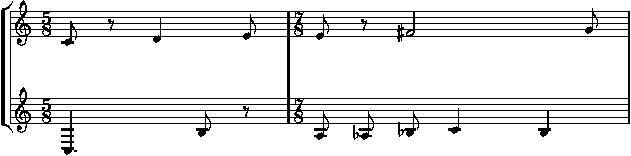
\includegraphics[max width=\textwidth,]{assets/lilypond-d1594e6b9d2ea25db305672b28ed63b4.pdf}
\end{singlespacing}
\end{abjadbookoutput}

\end{frame}

\begin{frame}[fragile]{Showing, playing, graphing components}
\begin{comment}
<abjad>
graph(score)
</abjad>
\end{comment}

\begin{abjadbookoutput}
\begin{singlespacing}
\vspace{-0.5\baselineskip}
\begin{minted}{pycon}
>>> graph(score)
\end{minted}
\noindent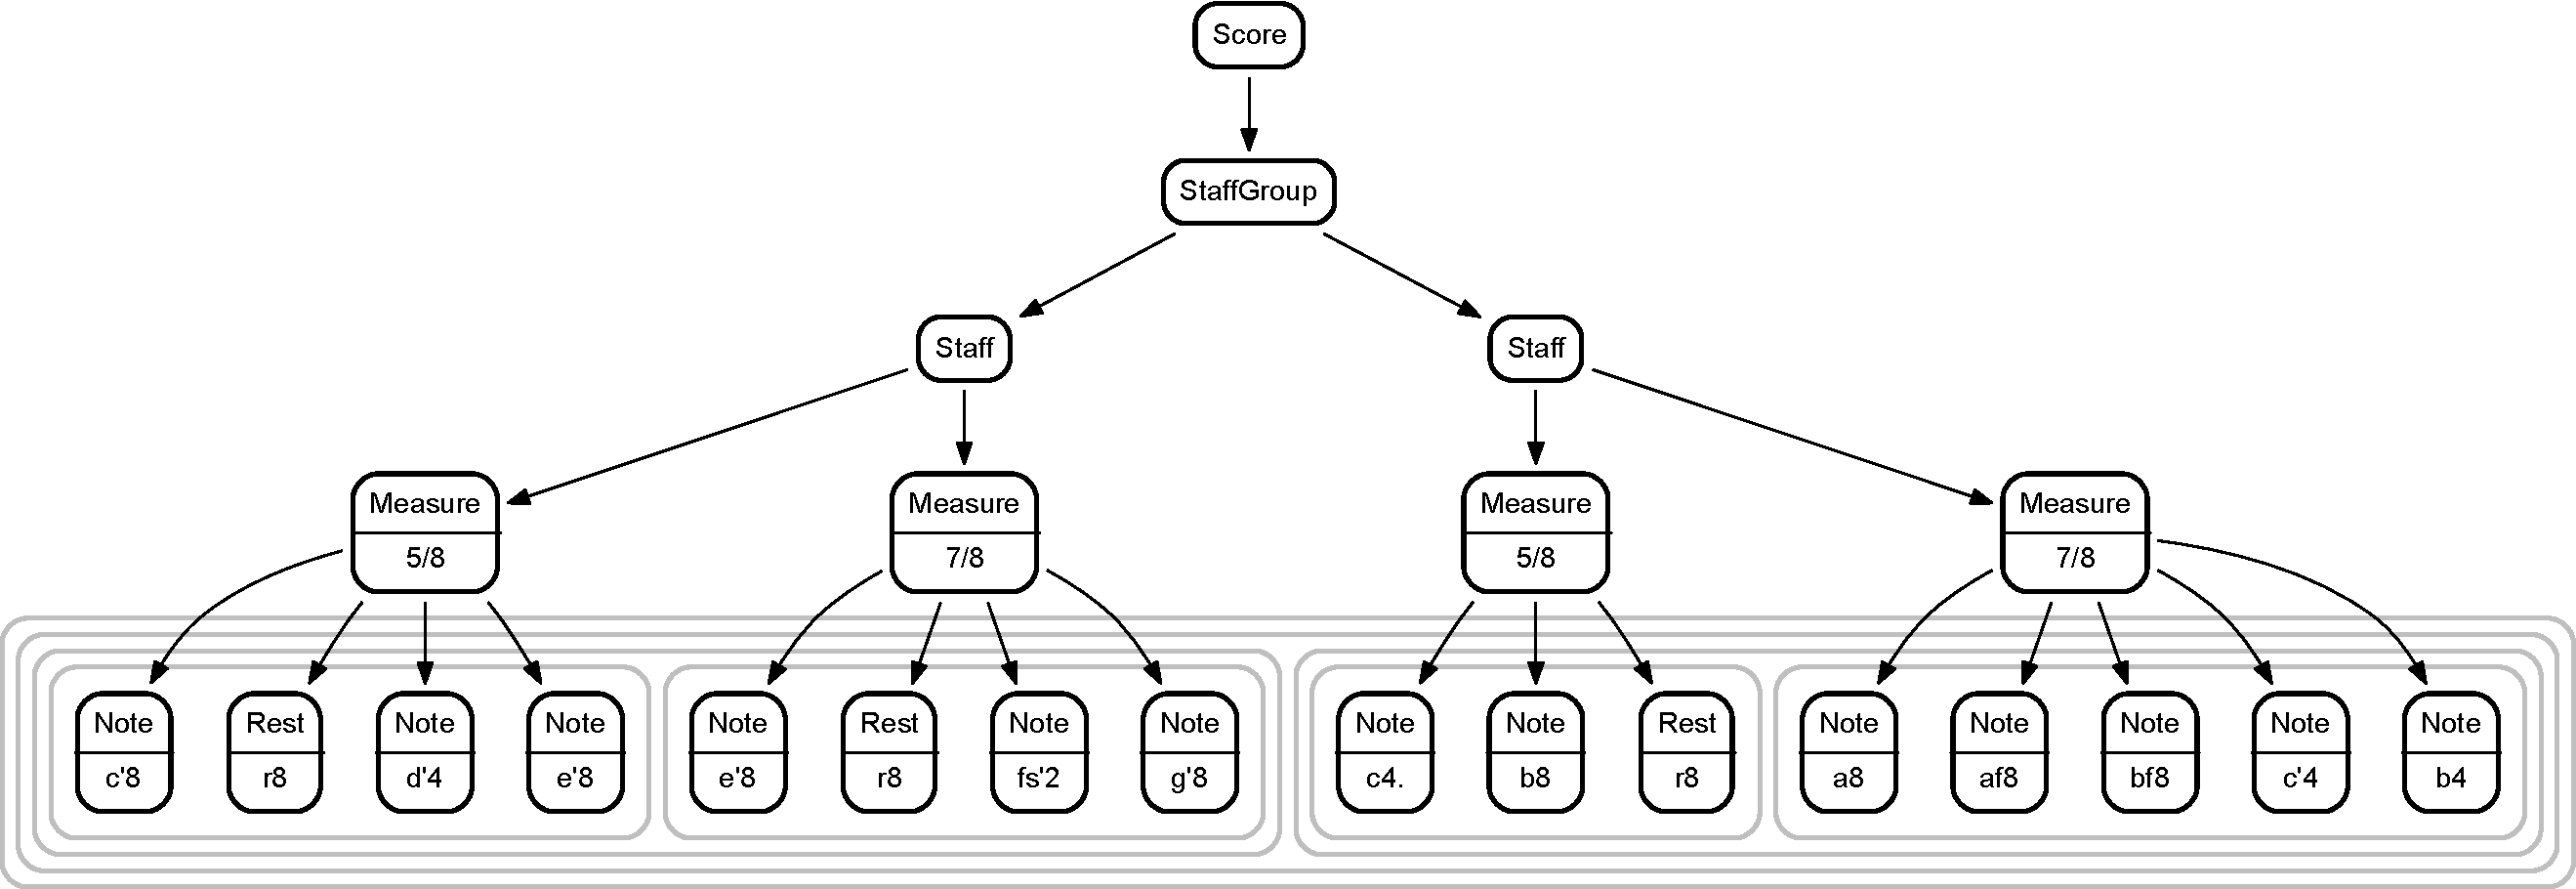
\includegraphics[scale=0.4,max width=\textwidth,]{assets/graphviz-e2d5b7f2bae136a90248b612d4d7243e.pdf}
\end{singlespacing}
\end{abjadbookoutput}

\end{frame}

\begin{frame}[fragile]{Attaching and detaching}
\begin{comment}
<abjad>
attach(Tempo((1, 4), 56), upper_staff[0][0])
attach(Hairpin('p < f'), upper_staff[:])
show(score)
</abjad>
\end{comment}

\begin{abjadbookoutput}
\begin{singlespacing}
\vspace{-0.5\baselineskip}
\begin{minted}{pycon}
>>> attach(Tempo((1, 4), 56), upper_staff[0][0])
>>> attach(Hairpin('p < f'), upper_staff[:])
>>> show(score)
\end{minted}
\noindent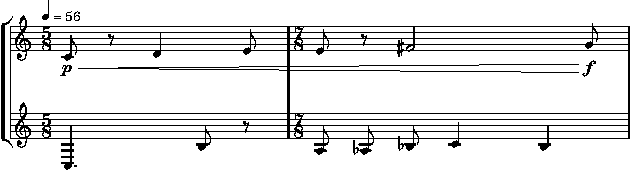
\includegraphics[max width=\textwidth,]{assets/lilypond-a9e19ad38171a32a9492dd585d335ca4.pdf}
\end{singlespacing}
\end{abjadbookoutput}

\end{frame}

\begin{frame}[fragile]{Inspecting components}
\end{frame}

\begin{frame}[fragile]{Indicator Scope}
\begin{markdown}
- Arbitrary objects can be attached to components
- They can be attached with *scope*
- Scoped objects *persist* until replaced
- Indicator scope can apply at different context levels
\end{markdown}
\begin{comment}
<abjad>
inspect_(score[0][1][1][4]).get_effective(Tempo)
</abjad>
\end{comment}

\begin{abjadbookoutput}
\begin{singlespacing}
\vspace{-0.5\baselineskip}
\begin{minted}{pycon}
>>> inspect_(score[0][1][1][4]).get_effective(Tempo)
Tempo(reference_duration=Duration(1, 4), units_per_minute=56)
\end{minted}
\end{singlespacing}
\end{abjadbookoutput}

\end{frame}

\begin{frame}[fragile]{Named components}
\end{frame}

\begin{frame}[fragile]{Iterating components}
\begin{comment}
<abjad>
iterator = iterate(score).by_timeline_and_logical_tie()
for index, logical_tie in enumerate(iterator):
    attach(Markup(index).circle(), logical_tie.head)

show(score)
</abjad>
\end{comment}

\begin{abjadbookoutput}
\begin{singlespacing}
\vspace{-0.5\baselineskip}
\begin{minted}{pycon}
>>> iterator = iterate(score).by_timeline_and_logical_tie()
>>> for index, logical_tie in enumerate(iterator):
...     attach(Markup(index).circle(), logical_tie.head)
...
>>> show(score)
\end{minted}
\noindent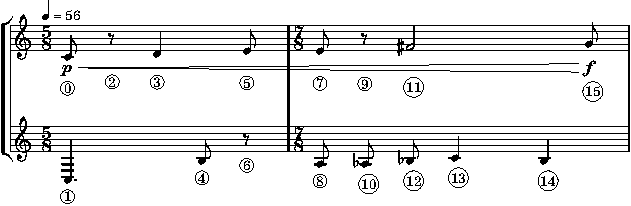
\includegraphics[max width=\textwidth,]{assets/lilypond-bac258cb0abf4373a16fc304b9b6d35b.pdf}
\end{singlespacing}
\end{abjadbookoutput}

\end{frame}

\begin{frame}[fragile]{Markup}
\end{frame}

\begin{frame}[fragile]{Component selectors}
*Selectors* provide JQuery-like logic for retrieving components
\end{frame}